\documentclass[french]{article}
\usepackage[T1]{fontenc}
\usepackage[utf8]{inputenc}
\usepackage{lmodern}
\usepackage[a4paper, margin=2.5cm]{geometry}
\usepackage{babel}
\usepackage[cache=false]{minted}
\usepackage{graphicx}
\usepackage{xcolor}
\usepackage{hyperref}
\definecolor{bg}{rgb}{0.98,0.98,0.98}

\title{Rapport Développement Logiciel}
\author{Badr YOUBI IDRISSI}

\begin{document}
\maketitle
\section{Introduction et fonctionnement général}

Dans ce projet nous codons un programme pour visualiser les isolignes 
d'un signal émit de plusieurs tétraèdres. 

\begin{figure}[h]
	\centering
	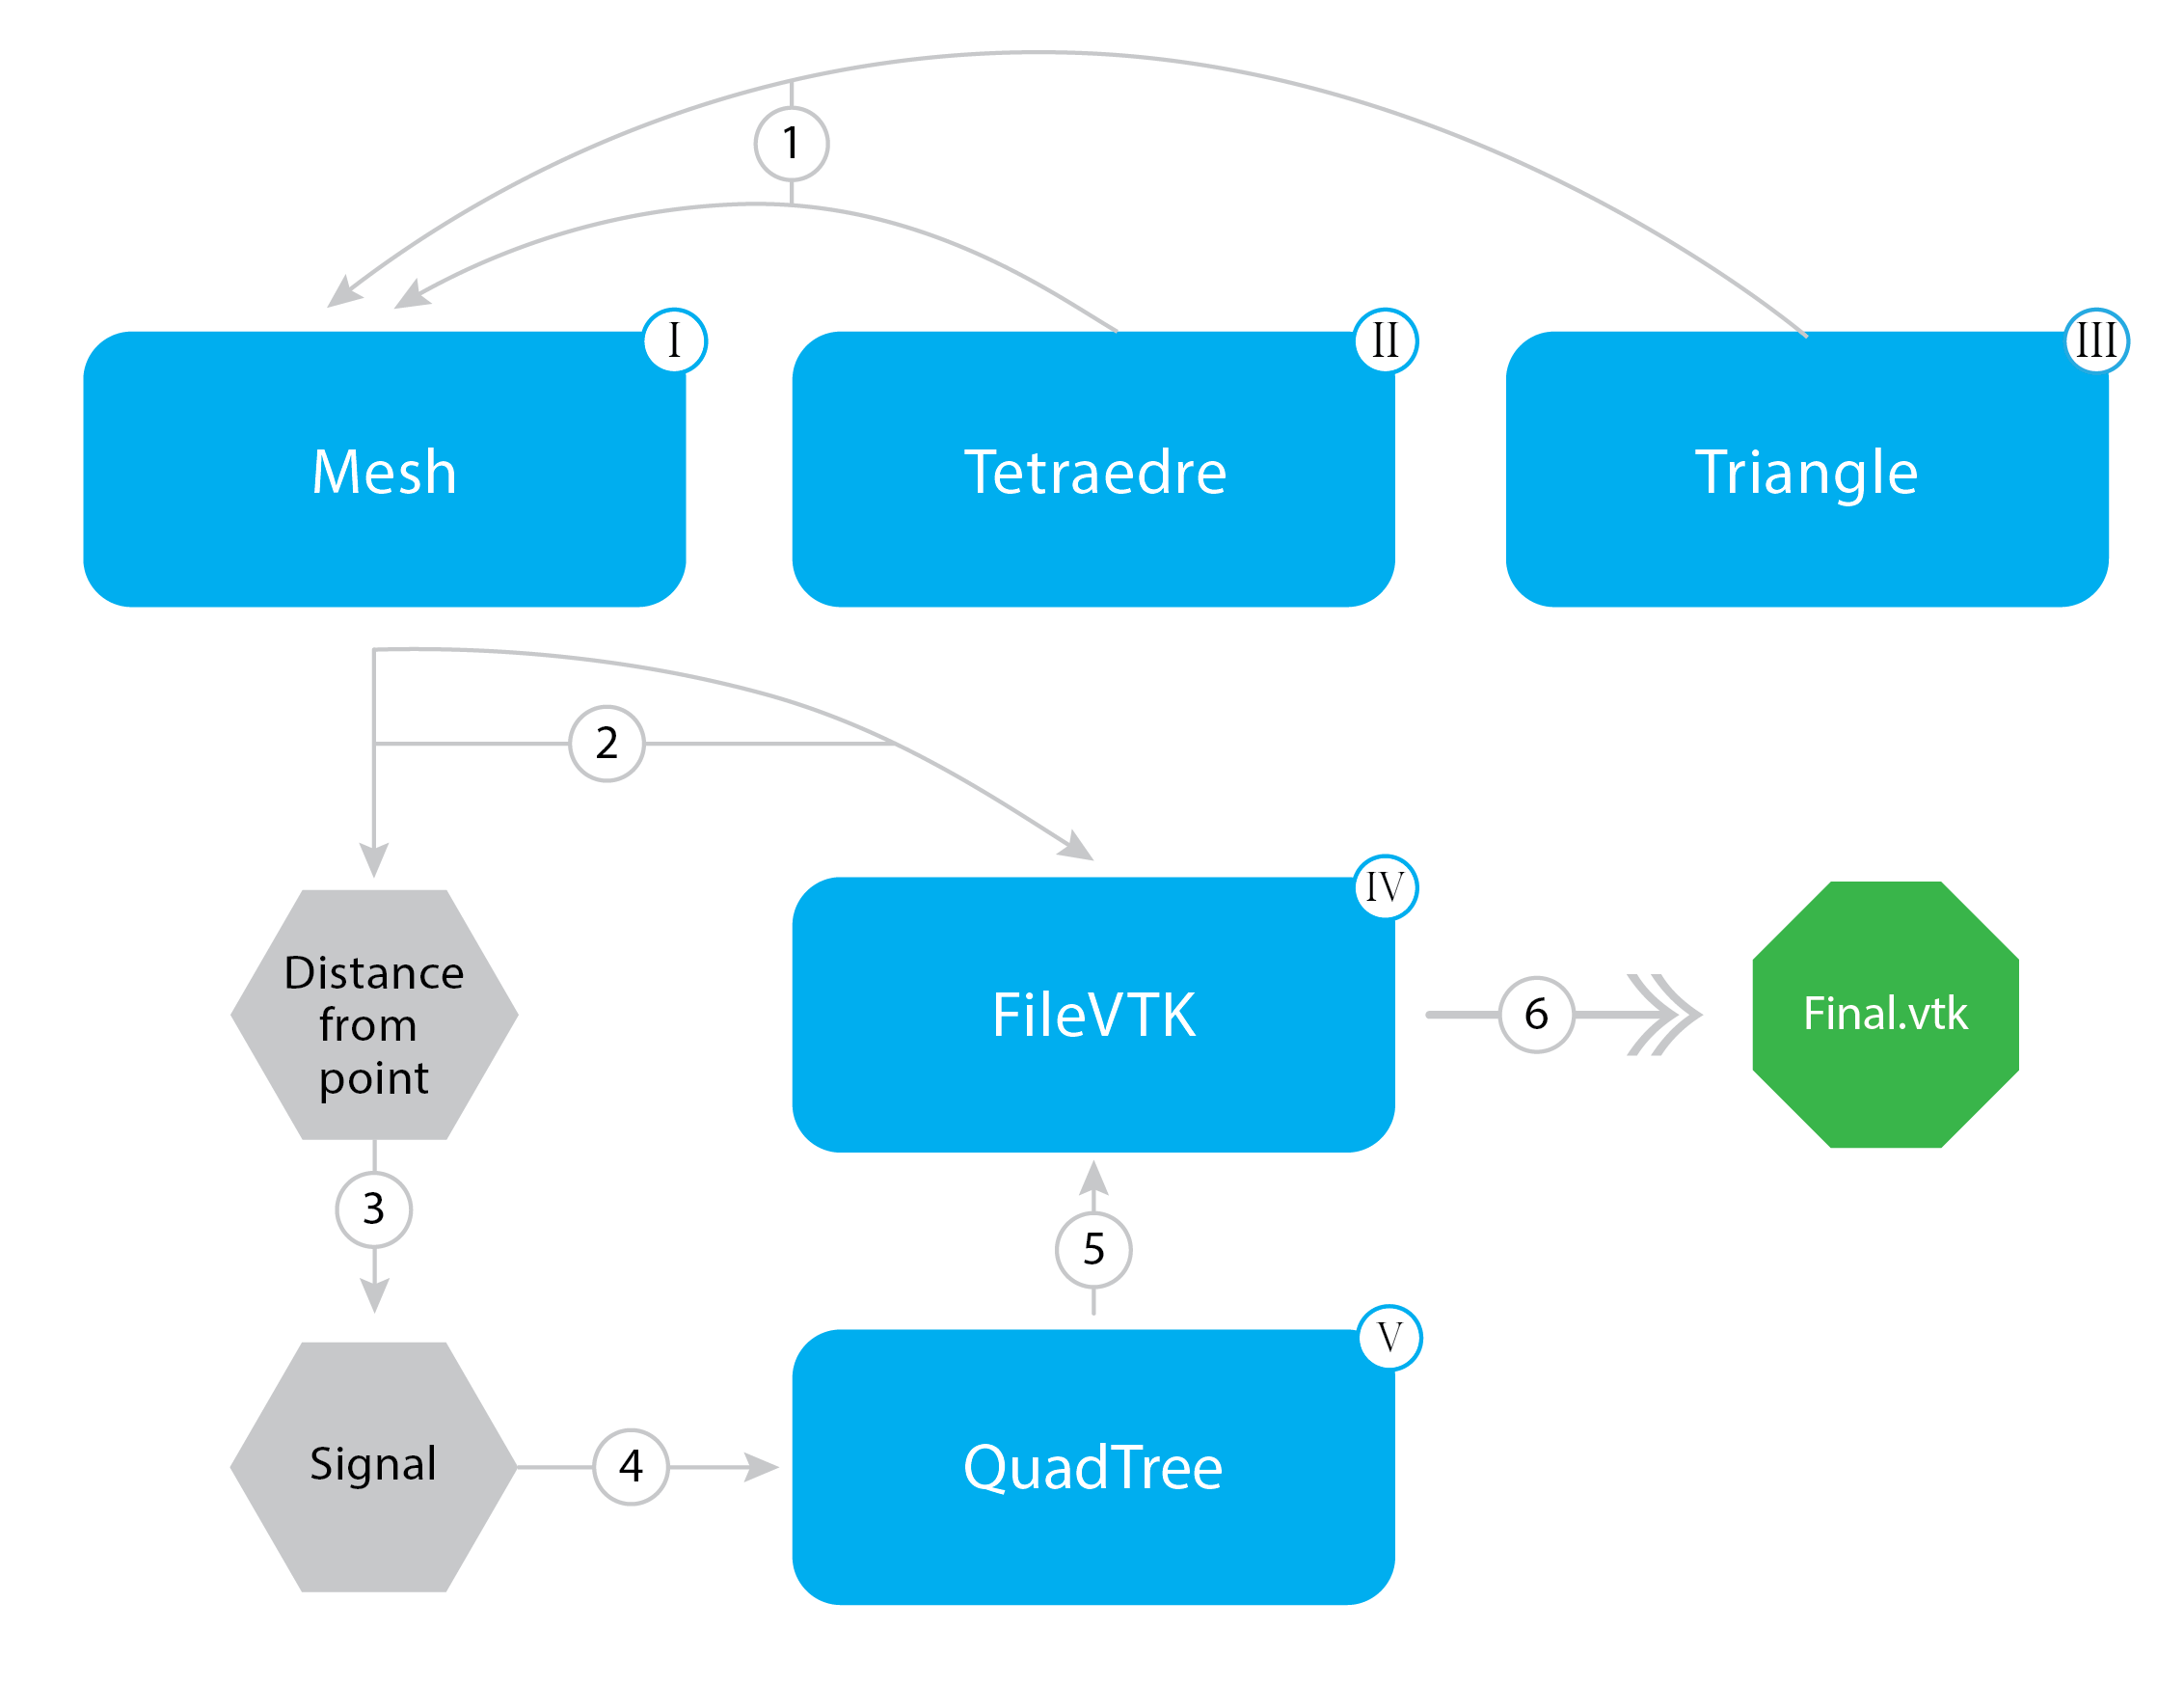
\includegraphics[width=0.7\textwidth]{Figures/SchemaNum.png}
	\caption{Schéma du fonctionnement général}
\end{figure}

On commence par créer l'objet 'Mesh' (\textit{I}) qui correspond à l'ensemble des pods émétant le signal.
L'objet mesh a besoin des points correspondant à chaque pod qui est un 'Tétraèdre' (\textit{II}) qui lui
même est un ensemble de 'Triangles' (\textit{III}) (\'Etape 1). Cet objet Mesh a la méthode distance from point qui 
renvoie la liste des distances entre un point et les pods (\'Etape 2). Ces distances servent ensuite à calculer le signal
en tout point de l'espace (\'Etape 3). on crée ensuite un plan à la hauteur 0.01 dont on va rafiner le maillage
avec l'objet 'QuadTree' (\textit{V}) (\'Etape 4). Ensuite l'ensemble des points et les valeurs du signal en ces points est
passé à l'objet 'FileVTK' (\textit{IV}) (\'Etape 5) qui va écrire le fichier "Final.vtk" (\'Etape 6).

\section{Description du code}
	
\subsection{Objet III : Triangle}
\vspace{10pt}
\begin{minted}[breakanywhere, xleftmargin=10pt]{python}

class tri:
	def __init__(self, point1, point2, point3): 
		...
	def distance_to_a_point(self, P): 
		...
\end{minted}

L'objet triangle sert à stocker les points du triangle et à calculer la distance entre
un point et à calculer la distance entre un point quelconque et le triangle.

\begin{minted}[breakanywhere, xleftmargin=10pt]{python}
def __init__(self, point1, point2, point3):
	self.points = [np.array(point1), np.array(point2), np.array(point3)]
	p1p2 = self.points[1]-self.points[0]
	p1p3 = self.points[2]-self.points[0]
	self.normal = np.cross(p1p2, p1p3)
	self.normal = self.normal/np.linalg.norm(self.normal)
\end{minted}
On enregistre les points A, B et C et on calcule la normale $ \overrightarrow{n'} = \overrightarrow{AB} \times \overrightarrow{AC} $
puis $ \vec{n} = \frac{\overrightarrow{n'}}{\|\overrightarrow{n'}\|} $

Pour la fonction de calcul de distance la fonction projète le point sur le plab du triangle puis selon 
les valeurs des coordonnées barycentriques on retourne la plus petite distance à un coin ou à un bord.
Au vu du grand nombre de cas, j'ai opté pour reprendre un code déjà fait qui applique ce principe 
(voir \href{run:https://gist.github.com/joshuashaffer/99d58e4ccbd37ca5d96e}{code}) en l'adaptant en rajoutant
la condition 
\begin{minted}[breakanywhere, xleftmargin=10pt]{python}
normal_side  = np.dot(self.normal, P) > np.dot(self.normal,self.points[0])
\end{minted}
car un point est du bon coté du plan du triangle si $ \langle\vec{p},\vec{n}\rangle > \langle\vec{A},\vec{n}\rangle $

\subsection{Objet II: Tetra}
\vspace{10pt}
\begin{minted}[breakanywhere, xleftmargin=10pt]{python}

class tetra:
	def __init__(self, point1, point2, point3, point4):
		...
	def distance_to_a_point(self, p):
		...

\end{minted}

L'objet tetra est un ensemble de triangles correctement orientés (normales vers l'extérieur) qui peut
calculer la distance entre un point et le tetra.
\begin{minted}[breakanywhere=true, xleftmargin=10pt]{python}
def __init__(self, point1, point2, point3, point4):
	self.points = [point1, point2,point3,point4]
	self.faces = [tri(point1,point3,point2), tri(point1,point4,point3),
				 tri(point2,point3,point4), tri(point1,point2,point4)]
\end{minted}
L'ordre des points ici est important pour bien orienter les normales.
\begin{figure}[h]
	\centering
	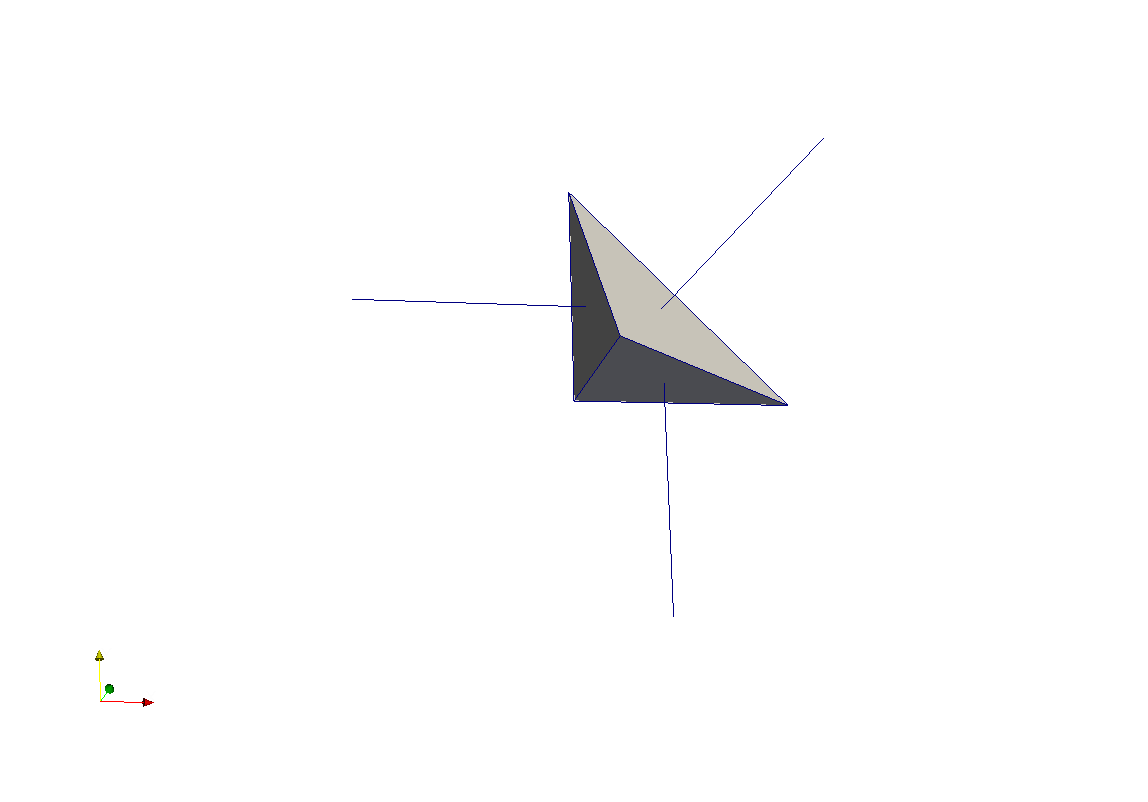
\includegraphics[width=0.7\textwidth]{Figures/TetraNormals.png}
	\caption{Tétraèdre avec normales}
\end{figure}

\begin{minted}[breakanywhere=true, xleftmargin=10pt]{python}
def distance_to_a_point(self, p):
	d_min = np.inf 
	outside = False
	
	for f in self.faces:
		[normal_side, d_minTri] = f.distance_to_a_point(p)
		outside = outside or normal_side
		if d_minTri < d_min:
			d_min = d_minTri
	
	return [outside, d_min] 
\end{minted}
la distance à un Tetraèdre est le minimum de distance aux autres triangles. sachant que si le point
est du mauvais côté la distance est infini.

\subsection{Objet I : mesh}
\vspace{10pt}
\begin{minted}[breakanywhere, xleftmargin=10pt]{python}

class tetra:
	def __init__ (self, DefenseFile):
		...
	def getNextValue(self)::
		...
	def toVector(self,string):
		...
	def radialVect(self,angle_in_degrees):
		...
	def Create_Mesh_And_Connectivity_List(self, List_Of_Point, Connectivity):
		...
	def Distance_Between_a_Point_and_the_Modules(self, p):
		...

\end{minted}

L'objet mesh génère des Tétraèdres à partir du fichier 'defense\_zone.txt' qui en donne les centres des bases équilatérales et
les hauteur. Les fonctions getNextValue, toVector et radialVect sont des fonctions auxiliaires.

\begin{minted}[xleftmargin=10pt]{python}
def __init__ (self, DefenseFile):
	self.List_Of_Modules = []
	self.file = open(DefenseFile)
	self.number_modules = int(self.getNextValue())
	
	for i in range(self.number_modules):
		center = self.toVector(self.getNextValue())
		base_length = float(self.getNextValue())
		height = float(self.getNextValue())
		rotation = float(self.getNextValue())
		i_z = np.array([0.0,0.0,1.0]) 
		
		distanceFromCenter = (np.sqrt(3)/3)*base_length
		point1 = center + self.radialVect(rotation)*distanceFromCenter
		point2 = center + self.radialVect(rotation + 120)*distanceFromCenter
		point3 = center + self.radialVect(rotation + 240)*distanceFromCenter
		point4 = center + height*i_z
		
		self.List_Of_Modules.append(tetra(point1, point2, point3, point4))

def getNextValue(self):
	return self.file.readline().strip().split(" : ")[1]

def radialVect(self,angle_in_degrees):
	i_x = np.array([1.0,0.0,0.0])
	i_y = np.array([0.0,1.0,0.0])
	return np.cos(angle_in_degrees*np.pi/180)*i_x + np.sin(angle_in_degrees*np.pi/180)*i_y


\end{minted}

Pour trouver les coordonnées du tétraèdres à partir des informations données on commence par
trouver la distance entre le centre et chacun des points de la base qui est égale
à $\frac{\sqrt{3}}{3}d$ avec d la longueur de la base. Le triangle est donc 3 points équidistants sur le cercle de rayon
$\frac{\sqrt{3}}{3}d$. On calcule le vecteur radial avec radialVect. getNextValue lit la ligne suivante et enlève le saut de ligne
et donne la valeur après les deux points.

\begin{minted}[xleftmargin=10pt]{python}
def Distance_Between_a_Point_and_the_Modules(self, p):

	outside = True
	d_min = []
	
	for t in self.List_Of_Modules:
		[outsidet, d_mint] = t.distance_to_a_point(p)
		outside = outside and outsidet
		d_min.append(d_mint)
	
	return [outside, np.array(d_min)]
\end{minted}

Cette fonction calcule la liste des distances et si oui ou non le points et dans un des pods.

\begin{figure}[h]
	\centering
	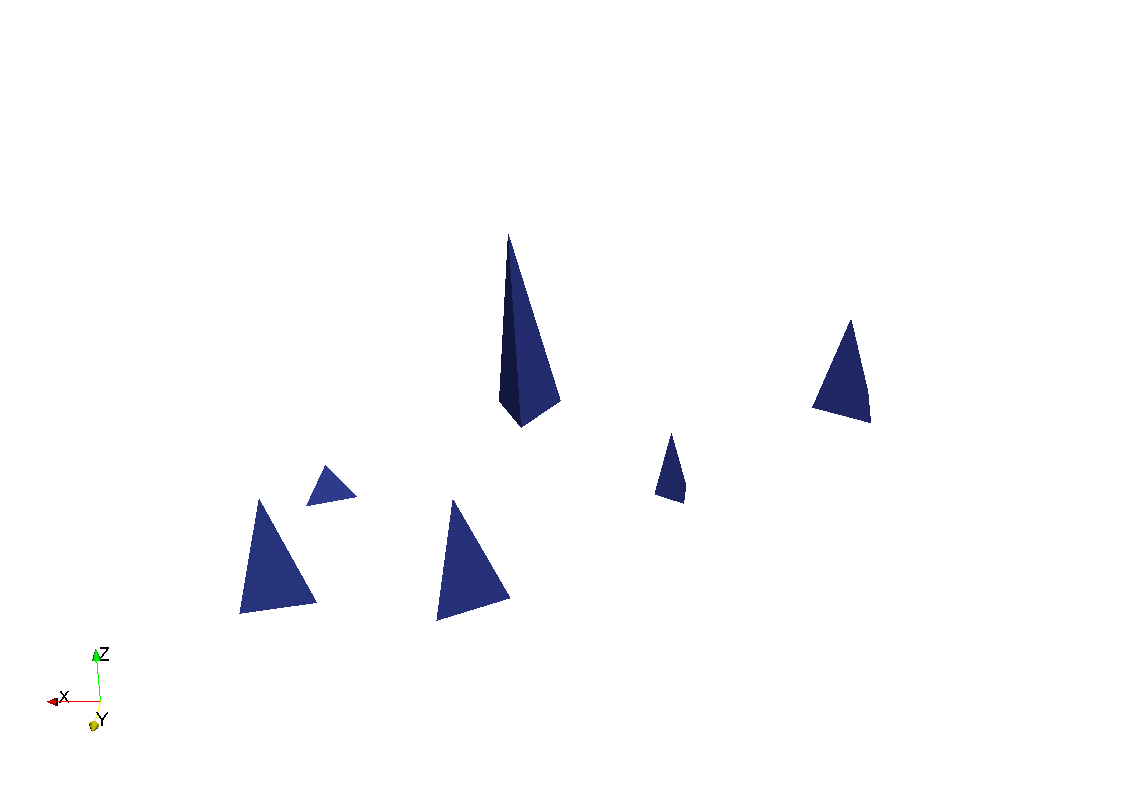
\includegraphics[width=0.7\textwidth]{Figures/Deffensezone.png}
	\caption{Objet mesh visualisé}
\end{figure}

\subsection{Objet V: QuadTree}

L'objet QuadTree est un objet qui raffine un maillage 2D selon les zones d'interêt.
\begin{minted}[xleftmargin=10pt]{python}
class tree_amr:
	def __init__(self, point_0, point_1, point_2, point_3, depth, depth_max, dico):
		...
	def Get_values(self, List_Of_Values):
		...
\end{minted}

Le gros du fonctionnement est dans l'initialisation :

\begin{minted}{python}

self.branch = False

#    store the information locally in the memory for the leaf 
self.point_0 = point_0
self.point_1 = point_1
self.point_2 = point_2
self.point_3 = point_3
self.depth_max = depth_max
self.depth = depth
self.dico = dico

r0 = self.dico['eval_function'](self.point_0,self.dico)
r1 = self.dico['eval_function'](self.point_1,self.dico)
r2 = self.dico['eval_function'](self.point_2,self.dico)
r3 = self.dico['eval_function'](self.point_3,self.dico)

self.val0 = r0
self.val1 = r1
self.val2 = r2
self.val3 = r3

if (depth < depth_max):

#   if the depth of the leaf is lower that the maximum depth 
#   then we check if we need to transform the leaf into a branch
#   We must transform the leaf into a branch 

  if self.dico['refine_or_not'](r0,r1,r2,r3, dico) or depth <= self.dico['level_min']:

  self.branch = True

  point_4 = (point_0+point_2) / 2
  point_5 = (point_0+point_1) / 2
  point_6 = (point_1+point_2) / 2
  point_7 = (point_2+point_3) / 2
  point_8 = (point_0+point_3) / 2

  self.child_up_left = tree_amr(point_8, point_4, point_7, point_3, depth+1, depth_max, dico)
  self.child_up_right = tree_amr(point_4, point_6, point_2, point_7, depth+1, depth_max, dico)
  self.child_down_left = tree_amr(point_0, point_5, point_4, point_8, depth+1, depth_max, dico)
  self.child_down_right = tree_amr(point_5, point_1, point_6, point_4, depth+1, depth_max, dico)

\end{minted}

On commence par calculer la fonction d'interêt en les coins puis on regarde si ces valeurs nous interessent
et si oui on crée récursivement des branches en subdivisant le plan en 4. Tout ceci en vérifiant qu'on ne
dépasse pas la profondeur maximale et qu'on dépasse au moins la profondeur minimale.

La fonction qui nous interesse ici est le signal en un point de l'espace. 

\begin{minted}{python}
def signal(p, dico):
    outside, d_min = dico['defZone'].Distance_Between_a_Point_and_the_Modules(p)
	if outside:
		return sum(1/d_min)
	else:
		return 2*max(isoligne)
\end{minted}

et la fonction qui définit si oui ou non le carré actuel est un point d'interêt est 

\begin{minted}{python}
def test_function(r0, r1, r2, r3, dico):
    cond = False
    for iso in dico['r_target']:
        cond = cond or ((r0 <  iso) | (r1 <  iso) | (r2 <  iso) | (r3 <  iso)) \
                        & ((r0 >= iso) | (r1 >= iso) | (r2 >= iso) | (r3 >= iso))
    return cond
\end{minted}

cette fonction regarde si la valeur d'une des isolignes est comprise entre les valeurs des coins du carré.

\end{document}
